

\tikzset{every picture/.style={line width=0.75pt}} %set default line width to 0.75pt        

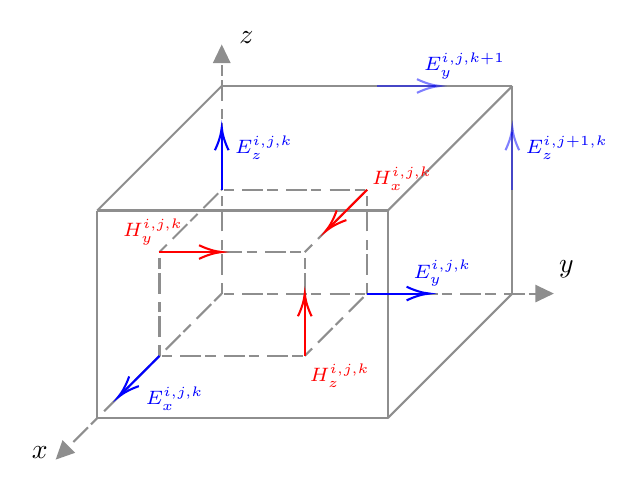
\begin{tikzpicture}[x=0.75pt,y=0.75pt,yscale=-1,xscale=1]
%uncomment if require: \path (0,300); %set diagram left start at 0, and has height of 300

%Straight Lines [id:da7206106706219195] 
\draw [color={rgb, 255:red, 142; green, 142; blue, 142 }  ,draw opacity=1 ]   (235,130) -- (235,30) ;
%Straight Lines [id:da33698179602076084] 
\draw [color={rgb, 255:red, 142; green, 142; blue, 142 }  ,draw opacity=1 ]   (35,190) -- (175,190) ;
%Straight Lines [id:da9138355462483165] 
\draw [color={rgb, 255:red, 142; green, 142; blue, 142 }  ,draw opacity=1 ]   (35,190) -- (35,90) ;
%Straight Lines [id:da685935512376388] 
\draw [color={rgb, 255:red, 142; green, 142; blue, 142 }  ,draw opacity=1 ]   (35,90) -- (175,90) ;
%Straight Lines [id:da445111134636218] 
\draw [color={rgb, 255:red, 142; green, 142; blue, 142 }  ,draw opacity=1 ]   (175,190) -- (235,130) ;
%Straight Lines [id:da484524333762936] 
\draw [color={rgb, 255:red, 142; green, 142; blue, 142 }  ,draw opacity=1 ]   (175,90) -- (235,30) ;
%Straight Lines [id:da9913295376298443] 
\draw [color={rgb, 255:red, 142; green, 142; blue, 142 }  ,draw opacity=1 ]   (35,90) -- (95,30) ;
%Straight Lines [id:da5460324336870037] 
\draw [color={rgb, 255:red, 142; green, 142; blue, 142 }  ,draw opacity=1 ]   (95,30) -- (235,30) ;
%Straight Lines [id:da6638914765185959] 
\draw [color={rgb, 255:red, 142; green, 142; blue, 142 }  ,draw opacity=1 ] [dash pattern={on 3.75pt off 3pt on 7.5pt off 1.5pt}]  (95,130) -- (95,13) ;
\draw [shift={(95,10)}, rotate = 90] [fill={rgb, 255:red, 142; green, 142; blue, 142 }  ,fill opacity=1 ][line width=0.08]  [draw opacity=0] (8.93,-4.29) -- (0,0) -- (8.93,4.29) -- cycle    ;
%Straight Lines [id:da5590643789875542] 
\draw [color={rgb, 255:red, 142; green, 142; blue, 142 }  ,draw opacity=1 ] [dash pattern={on 3.75pt off 3pt on 7.5pt off 1.5pt}]  (96,130) -- (252,130) ;
\draw [shift={(255,130)}, rotate = 180] [fill={rgb, 255:red, 142; green, 142; blue, 142 }  ,fill opacity=1 ][line width=0.08]  [draw opacity=0] (8.93,-4.29) -- (0,0) -- (8.93,4.29) -- cycle    ;
%Straight Lines [id:da13059528999125825] 
\draw [color={rgb, 255:red, 142; green, 142; blue, 142 }  ,draw opacity=1 ] [dash pattern={on 3.75pt off 3pt on 7.5pt off 1.5pt}]  (17.12,207.88) -- (95,130) ;
\draw [shift={(15,210)}, rotate = 315] [fill={rgb, 255:red, 142; green, 142; blue, 142 }  ,fill opacity=1 ][line width=0.08]  [draw opacity=0] (8.93,-4.29) -- (0,0) -- (8.93,4.29) -- cycle    ;
%Straight Lines [id:da6668538193606308] 
\draw [color={rgb, 255:red, 142; green, 142; blue, 142 }  ,draw opacity=1 ]   (175,190) -- (175,90) ;
%Straight Lines [id:da383295540871357] 
\draw [color={rgb, 255:red, 142; green, 142; blue, 142 }  ,draw opacity=1 ] [dash pattern={on 3.75pt off 3pt on 7.5pt off 1.5pt}]  (165,130) -- (165,80) ;
%Straight Lines [id:da3974993340565597] 
\draw [color={rgb, 255:red, 142; green, 142; blue, 142 }  ,draw opacity=1 ] [dash pattern={on 3.75pt off 3pt on 7.5pt off 1.5pt}]  (65,160) -- (65,110) ;
%Straight Lines [id:da44160642910672465] 
\draw [color={rgb, 255:red, 142; green, 142; blue, 142 }  ,draw opacity=1 ] [dash pattern={on 3.75pt off 3pt on 7.5pt off 1.5pt}]  (135,160) -- (135,110) ;
%Straight Lines [id:da5629234248062879] 
\draw [color={rgb, 255:red, 142; green, 142; blue, 142 }  ,draw opacity=1 ] [dash pattern={on 3.75pt off 3pt on 7.5pt off 1.5pt}]  (66,160) -- (135,160) ;
%Straight Lines [id:da5422854229817635] 
\draw [color={rgb, 255:red, 142; green, 142; blue, 142 }  ,draw opacity=1 ] [dash pattern={on 3.75pt off 3pt on 7.5pt off 1.5pt}]  (65,110) -- (135,110) ;
%Straight Lines [id:da6116059635293223] 
\draw [color={rgb, 255:red, 142; green, 142; blue, 142 }  ,draw opacity=1 ] [dash pattern={on 3.75pt off 3pt on 7.5pt off 1.5pt}]  (96,80) -- (165,80) ;
%Straight Lines [id:da9246979014557115] 
\draw [color={rgb, 255:red, 142; green, 142; blue, 142 }  ,draw opacity=1 ] [dash pattern={on 3.75pt off 3pt on 7.5pt off 1.5pt}]  (65,110) -- (95,80) ;
%Straight Lines [id:da7936751206446481] 
\draw [color={rgb, 255:red, 142; green, 142; blue, 142 }  ,draw opacity=1 ] [dash pattern={on 3.75pt off 3pt on 7.5pt off 1.5pt}]  (135,110) -- (165,80) ;
%Straight Lines [id:da5136819716767439] 
\draw [color={rgb, 255:red, 142; green, 142; blue, 142 }  ,draw opacity=1 ] [dash pattern={on 3.75pt off 3pt on 7.5pt off 1.5pt}]  (135,160) -- (165,130) ;
%Straight Lines [id:da7961144391033157] 
\draw [color={rgb, 255:red, 255; green, 0; blue, 0 }  ,draw opacity=1 ]   (65,110) -- (93,110) ;
\draw [shift={(95,110)}, rotate = 180] [color={rgb, 255:red, 255; green, 0; blue, 0 }  ,draw opacity=1 ][line width=0.75]    (10.93,-3.29) .. controls (6.95,-1.4) and (3.31,-0.3) .. (0,0) .. controls (3.31,0.3) and (6.95,1.4) .. (10.93,3.29)   ;
%Straight Lines [id:da12124972293983005] 
\draw [color={rgb, 255:red, 255; green, 0; blue, 0 }  ,draw opacity=1 ]   (165,80) -- (146.41,98.59) ;
\draw [shift={(145,100)}, rotate = 315] [color={rgb, 255:red, 255; green, 0; blue, 0 }  ,draw opacity=1 ][line width=0.75]    (10.93,-3.29) .. controls (6.95,-1.4) and (3.31,-0.3) .. (0,0) .. controls (3.31,0.3) and (6.95,1.4) .. (10.93,3.29)   ;
%Straight Lines [id:da3302622370080578] 
\draw [color={rgb, 255:red, 255; green, 0; blue, 0 }  ,draw opacity=1 ]   (135,160) -- (135,132) ;
\draw [shift={(135,130)}, rotate = 90] [color={rgb, 255:red, 255; green, 0; blue, 0 }  ,draw opacity=1 ][line width=0.75]    (10.93,-3.29) .. controls (6.95,-1.4) and (3.31,-0.3) .. (0,0) .. controls (3.31,0.3) and (6.95,1.4) .. (10.93,3.29)   ;
%Straight Lines [id:da5288808191623237] 
\draw [color={rgb, 255:red, 0; green, 0; blue, 255 }  ,draw opacity=1 ]   (95,80) -- (95,52) ;
\draw [shift={(95,50)}, rotate = 90] [color={rgb, 255:red, 0; green, 0; blue, 255 }  ,draw opacity=1 ][line width=0.75]    (10.93,-3.29) .. controls (6.95,-1.4) and (3.31,-0.3) .. (0,0) .. controls (3.31,0.3) and (6.95,1.4) .. (10.93,3.29)   ;
%Straight Lines [id:da13848590216057788] 
\draw [color={rgb, 255:red, 0; green, 0; blue, 255 }  ,draw opacity=1 ]   (65,160) -- (46.41,178.59) ;
\draw [shift={(45,180)}, rotate = 315] [color={rgb, 255:red, 0; green, 0; blue, 255 }  ,draw opacity=1 ][line width=0.75]    (10.93,-3.29) .. controls (6.95,-1.4) and (3.31,-0.3) .. (0,0) .. controls (3.31,0.3) and (6.95,1.4) .. (10.93,3.29)   ;
%Straight Lines [id:da9041413940467059] 
\draw [color={rgb, 255:red, 0; green, 0; blue, 255 }  ,draw opacity=1 ]   (165,130) -- (193,130) ;
\draw [shift={(195,130)}, rotate = 180] [color={rgb, 255:red, 0; green, 0; blue, 255 }  ,draw opacity=1 ][line width=0.75]    (10.93,-3.29) .. controls (6.95,-1.4) and (3.31,-0.3) .. (0,0) .. controls (3.31,0.3) and (6.95,1.4) .. (10.93,3.29)   ;
%Straight Lines [id:da7338603939817645] 
\draw [color={rgb, 255:red, 0; green, 0; blue, 255 }  ,draw opacity=0.5 ]   (170,30) -- (198,30) ;
\draw [shift={(200,30)}, rotate = 180] [color={rgb, 255:red, 0; green, 0; blue, 255 }  ,draw opacity=0.5 ][line width=0.75]    (10.93,-3.29) .. controls (6.95,-1.4) and (3.31,-0.3) .. (0,0) .. controls (3.31,0.3) and (6.95,1.4) .. (10.93,3.29)   ;
%Straight Lines [id:da686817746379393] 
\draw [color={rgb, 255:red, 0; green, 0; blue, 255 }  ,draw opacity=0.5 ]   (235,80) -- (235,52) ;
\draw [shift={(235,50)}, rotate = 90] [color={rgb, 255:red, 0; green, 0; blue, 255 }  ,draw opacity=0.5 ][line width=0.75]    (10.93,-3.29) .. controls (6.95,-1.4) and (3.31,-0.3) .. (0,0) .. controls (3.31,0.3) and (6.95,1.4) .. (10.93,3.29)   ;

% Text Node
\draw (2,202.4) node [anchor=north west][inner sep=0.75pt]    {$x$};
% Text Node
\draw (256,112.4) node [anchor=north west][inner sep=0.75pt]    {$y$};
% Text Node
\draw (102,2.4) node [anchor=north west][inner sep=0.75pt]    {$z$};
% Text Node
\draw (46,92.4) node [anchor=north west][inner sep=0.75pt]  [font=\scriptsize,color={rgb, 255:red, 255; green, 0; blue, 0 }  ,opacity=1 ]  {$H_{y}^{i,j,k}$};
% Text Node
\draw (136,162.4) node [anchor=north west][inner sep=0.75pt]  [font=\scriptsize,color={rgb, 255:red, 255; green, 0; blue, 0 }  ,opacity=1 ]  {$H_{z}^{i,j,k}$};
% Text Node
\draw (166,67.4) node [anchor=north west][inner sep=0.75pt]  [font=\scriptsize,color={rgb, 255:red, 255; green, 0; blue, 0 }  ,opacity=1 ]  {$H_{x}^{i,j,k}$};
% Text Node
\draw (57,173.4) node [anchor=north west][inner sep=0.75pt]  [font=\scriptsize,color={rgb, 255:red, 0; green, 0; blue, 255 }  ,opacity=1 ]  {$E_{x}^{i,j,k}$};
% Text Node
\draw (186,112.4) node [anchor=north west][inner sep=0.75pt]  [font=\scriptsize,color={rgb, 255:red, 0; green, 0; blue, 255 }  ,opacity=1 ]  {$E_{y}^{i,j,k}$};
% Text Node
\draw (100,52.4) node [anchor=north west][inner sep=0.75pt]  [font=\scriptsize,color={rgb, 255:red, 0; green, 0; blue, 255 }  ,opacity=1 ]  {$E_{z}^{i,j,k}$};
% Text Node
\draw (191,12.4) node [anchor=north west][inner sep=0.75pt]  [font=\scriptsize,color={rgb, 255:red, 0; green, 0; blue, 255 }  ,opacity=1 ]  {$E_{y}^{i,j,k+1}$};
% Text Node
\draw (240,52.4) node [anchor=north west][inner sep=0.75pt]  [font=\scriptsize,color={rgb, 255:red, 0; green, 0; blue, 255 }  ,opacity=1 ]  {$E_{z}^{i,j+1,k}$};


\end{tikzpicture}
